\section{Einführung \tiny (Vorlesung 1 am 17.10.)}
\subsection{Organisatorisches}
Mitschrift wird von Studenten erstellt.\\

Korrekturfarbe für Gummipunkte: Grün!\\

\subsection*{Voraussetzungen}
\begin{itemize}
\item O-Notation
\item Turing-Maschine
\item Sortieralgorithmen
\item Schubfachprinzip
\item Gauß-Nummer
\item Harmonische Reihe
\end{itemize}
\subsection{Kuchen teilen}

\textbf{Problem:} Ein Kuchen soll unter zwei Personen aufgeteilt werden.\\
Zwei Lösungsideen: 
\begin{compactitem}
\item perfektes Teilen
\item einer teilt den Kuchen und der andere sucht sich eine Hälfte aus.
\end{compactitem}
Was passiert, wenn jemand die Teile des Kuchens unterschiedlich bewertet? (z.B. Kirsche auf einer Seite, viel Sahne auf der anderen Seite)\\
Perfektes teilen bedeutet, dass jemand \emph{für sich} perfekt teilt. (nach seinem Maßstab)\\
\textbf{Ziel: Fairness} Jeder will $\frac{1}{n}$ des Kuchens nach ihrem Maßstab. ($n=\#$Personen)
\subsubsection{1. Algorithmus (für 2 Personen)}
\begin{enumerate}
\item Erste teilt
\item Zweite sucht aus
\end{enumerate}
Der Algorithmus ist toll, aber es gibt zu viele Schritte. Daher wollen wir den Algorithmus verbessern.\\
\textbf{Ziel:} möglichst wenige \underline{Schritte}.
\subsubsection{2. Algorithmus (für 3 Personen)}
Anton, Berta und Clara:
\begin{enumerate}
	\item Anton teilt $\frac{1}{3} | \frac{2}{3}$
	\item Berta teilt $\frac{\frac{2}{3}}{2}|\frac{\frac{2}{3}}{2}$
	\item Clara sucht aus.
	\item Anton sucht aus.
	\begin{enumerate}
		\item [Fall 1:] Clara nimmt eines der rechten Stücke $\Rightarrow$ Anton nimmt linkes Stück.
		\item [Fall 2:] Clara nimmt linkes Stück.\\ Schubfachprinzip: eines der rechten Stücke ist mindestens $\frac{1}{3}$
	\end{enumerate}
	\item Berta ):
\end{enumerate}
\subsubsection{3. Teilen und Trimmen}
\begin{enumerate}
	\item Anton teilt:
	%gfx
	\begin{figure}[h]
	\centering
	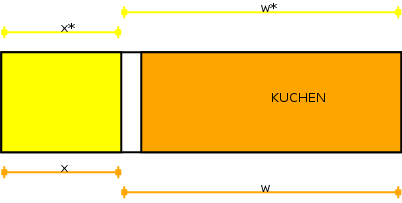
\includegraphics[width=300px]{../GFX/teilenundtrimmen.png}
\end{figure}
	\item Berta:
	\begin{enumerate}
		\item[Fall 1:] Berta denkt $x \leq \frac{1}{3}$
		\item[Fall 2:] Berta denkt $x > \frac{1}{3} \Rightarrow$ Trimmen
	\end{enumerate}
	\item Clara darf sich entscheiden:
		\begin{enumerate}
		\item[Fall 1:] will $x^*$ dann Algorithmus 1. für den Rest 
		\item[Fall 2:] will $x^*$ nicht.\\$\Rightarrow w^* \geq \frac{2}{3}$ für Clara und Anton\\
	\end{enumerate}
\end{enumerate}
\subsubsection{4. Teilen mit bewegtem Messer}
% gfx Kuchen mit Messer
Man nimmt ein Messer und jede Person sagt einfach Stop, wenn die \emph{perfekte Wahl} für die Person getroffen ist.\\
$\#$Schritte $= n-1$
\subsubsection{5. Simuliertes bewegtes Messer}
\begin{itemize}
	\item Jeder macht bei $\frac{1}{n}$ eine Markierung
	\item der/die Linkeste bekommt das Stück\\$\#$Schritte $=n+(n-1)+...3+2=\theta(n^2)$ (Gauß-Nummer)
\end{itemize}
\subsubsection{6. Simuliertes Messer + Zufall}
Wie 5., aber
\begin{enumerate}
	\item Reihenfolge zufällig
	\item nur neue Linkeste Markierung werden gemacht
	%TODO Mathalign
	\item $T(n) = \#$erwartete Markierungen\\
	$= \underbrace{\frac{1}{n}}_{\text{Erwartete Anzahl der letzten Markierung}} + \underbrace{T(n-1)}_{\text{Erwartete Anzahl von Markierungen aller Anderen.}}$
	\item $T(n)=1+\frac{1}{2}+\frac{1}{3}+\frac{1}{4}+\dots+\frac{1}{n} = \theta(\log n)$ (harmonische Reihe)
	\item Gesamtlaufzeit $\leq n * O(\log n) = O(n * \log n)$
\end{enumerate}
\subsubsection{7. Divide \& Conquer}
$n$ Personen\\
$n$ Markierungen bei $\frac{k}{n}$\\
$\#$Schritte im Worst Case $T(n) = n +2$

\subsubsection{8. Divde \& Conquer + Zufall}
(erwartete) Laufzeit pro Teilen $\theta (\log n)$ also insgesamt $\theta(n)$